 \documentclass[12pt]{article}
 \usepackage{cancel}
 \usepackage{multicol}
 \usepackage{amsmath}
 \usepackage{amssymb}
 \usepackage{setspace}
 \usepackage{xcolor}
 \usepackage{graphicx}    % needed for including graphics e.g. EPS, PS
 \usepackage{tikz}
 \usetikzlibrary{patterns,decorations.pathreplacing,shapes,arrows,matrix,positioning}
 \usepackage{3dplot}
 \usepackage[vlined]{algorithm2e}
 \topmargin -2.5cm        % read Lamport p.163
 \oddsidemargin -0.04cm   % read Lamport p.163
 \evensidemargin -0.04cm  % same as oddsidemargin but for left-hand pages
 \textwidth 16.59cm
 \textheight 25.94cm
% \pagestyle{empty}        % Uncomment if don't want page numbers
 \pagenumbering{gobble}
 \parskip 7.2pt           % sets spacing between paragraphs
 %\renewcommand{\baselinestretch}{1.5} 	% Uncomment for 1.5 spacing between lines
 \parindent 0pt		  % sets leading space for paragraphs

% Title
\title{\LARGE\textbf{Chapter 8: Eigenvalues}\normalsize}

% No date in header
\date{}

\newcommand{\inv}[1]{{#1}^{-1}}

\newcommand{\iter}[1]{^{\myp{#1}}}

\newcommand{\lp}{\left(}
\newcommand{\rp}{\right)}
\newcommand{\lb}{\left[}
\newcommand{\rb}{\right]}
\newcommand{\ls}{\left\{}
\newcommand{\rs}{\right\}}
\newcommand{\lbar}{\left|}
\newcommand{\rbar}{\right|}
\newcommand{\ld}{\left.}
\newcommand{\rd}{\right.}

\newcommand{\hs}{\hspace{.75mm}}
\newcommand{\bs}{\hspace{-.75mm}}
\newcommand{\nin}{\noindent}

\newcommand{\fx}{f\bs\left( x \right)}
\newcommand{\gx}{g\bs\left( x \right)}
\newcommand{\qx}{q\bs\left( x \right)}

\newcommand{\nn}{\nonumber}

\newcommand{\vfive}{\vspace{5mm}}
\newcommand{\vthree}{\vspace{3mm}}

\newcommand{\fof}[1]{f\lp #1\rp}
\newcommand{\gof}[1]{g\lp #1\rp}
\newcommand{\qof}[1]{q\lp #1\rp}

\newcommand{\myp}[1]{\left( #1 \right)}
\newcommand{\myb}[1]{\left[ #1 \right]}
\newcommand{\myv}[1]{\left< #1 \right>}
\newcommand{\mys}[1]{\left\{ #1 \right\}}
\newcommand{\myab}[1]{\left| #1 \right|}

\newcommand{\myj}{_j}
\newcommand{\myjp}{_{j+1}}
\newcommand{\myjm}{_{j-1}}

\newcommand{\f}[1]{f\hspace{-1mm}\left( #1 \right)}
\newcommand{\fp}[1]{f'\hspace{-1mm}\left( #1 \right)}
\newcommand{\g}[1]{g\hspace{-1mm}\left( #1 \right)}
\newcommand{\gp}[1]{g'\hspace{-1mm}\left( #1 \right)}
\newcommand{\q}[1]{q\hspace{-1mm}\left( #1 \right)}
\newcommand{\qp}[1]{q'\hspace{-1mm}\left( #1 \right)}
\newcommand{\Px}[1]{P\hspace{-1mm}\left( x_{#1} \right)}
\newcommand{\Qx}[1]{Q\hspace{-1mm}\left( x_{#1} \right)}

\newcommand{\tten}[1]{\times 10^{#1}}

\newcommand{\aij}[1]{a_{#1}}
\newcommand{\bij}[1]{b_{#1}}

\newcommand{\R}[1]{\mathbb{R}^{#1}}
\newcommand{\C}[1]{\mathbb{C}^{#1}}
\newcommand{\F}[1]{\mathbb{F}^{#1}}
\newcommand{\myr}[1]{\textcolor{red}{#1}}

\newcommand{\ith}{i^{\textrm{th}}}
\newcommand{\jth}{j^{\textrm{th}}}
\newcommand{\kth}{k^{\textrm{th}}}

\newcommand{\ben}{\begin{enumerate}}
\newcommand{\een}{\end{enumerate}}

\newcommand{\beq}{\begin{eqnarray}}
\newcommand{\eeq}{\end{eqnarray}}

\tikzset{>=stealth'}

% matrix macro
\newcommand{\mymat}[1]{
\left[
\begin{array}{rrrrrrrrrrrrrrrrrrrrrrrrrrrrrrrrrrrrrrr}
#1
\end{array}
\right]
}

\newcommand{\mydet}[1]{
\left|
\begin{array}{rrrrrrrrrrrrrrrrrrrrrrrrrrrrrrrrrrrrrrr}
#1
\end{array}
\right|
}

\newcommand{\mydim}[2]{
$#1 \times #2$
}

\newcommand{\myra}{\quad \Rightarrow \quad}

\newcommand{\bS}{\mathbf{S}}
\newcommand{\bw}{\mathbf{w}}
\newcommand{\bx}{\mathbf{x}}
\newcommand{\bX}{\mathbf{X}}
\newcommand{\bd}{\mathbf{d}}
\newcommand{\bdx}{\mathbf{\delta x}}
\newcommand{\bp}{\mathbf{p}}
\newcommand{\bq}{\mathbf{q}}
\newcommand{\bz}{\mathbf{z}}
\newcommand{\bv}{\mathbf{v}}
\newcommand{\bu}{\mathbf{u}}
\newcommand{\by}{\mathbf{y}}
\newcommand{\ba}{\mathbf{a}}
\newcommand{\bb}{\mathbf{b}}
\newcommand{\bc}{\mathbf{c}}
\newcommand{\be}{\mathbf{e}}
\newcommand{\br}{\mathbf{r}}
\newcommand{\bh}{\mathbf{h}}
\newcommand{\bfb}{\mathbf{b}}
\newcommand{\xhat}{\hat{\mathbf{x}}}
\newcommand{\bzero}{\mathbf{0}}

\newcommand{\coker}{\textrm{coker}\hs}
\newcommand{\corange}{\textrm{corng}\hs}
\newcommand{\range}{\textrm{rng}\hs}
\newcommand{\myspan}{\textrm{span}\hs}
\newcommand{\rank}{\textrm{rank}\hs}
\newcommand{\trace}{\textrm{tr}\hs}

\newcommand{\lam}{\lambda}


\tikzstyle{block} = [rectangle, draw, fill=blue!15, text width=6em, text centered, rounded corners, minimum height=4em]
\tikzstyle{line} = [draw, -latex']

\tikzset{main node/.style={circle,fill=blue!20,draw,minimum size=.75cm,inner sep=0pt},
            }

% Actual document starts here
% ======================================================================================
\begin{document}
% \maketitle

% Footer
\let\thefootnote\relax\footnotetext{
\\ Chris Ketelsen
\\ CSCI 2820
\\ Graphics Transformations
\\ \today }

\tdplotsetmaincoords{60}{120}

% Actual text body starts here
% ======================================================================================

\vspace{-15mm}

% =================================================================================================================
% Lecture 23: 2D graphics transformations
% =================================================================================================================

\nin\Huge{\bf Graphics Transformations}\normalsize
\vspace{4mm}
\hrule

\vspace{5mm}

\nin Computer graphics are are images displayed or animated on a computer screen.  Computer graphics are used all over the web, in video games, and computer aided design (CAD) systems.  At it's core, computer graphics are the manipulation of points and shapes.  Most of the shapes are approximated by straight lines or polygons.  In this lecture and the next we'll look at how you can formulate the manipulation of basic shapes as a set of linear transformations.  We'll start with graphics in 2D and then extend the tools we develop to 3D.  %Finally we'll talk about how a 3D shape or set of shapes is produced onto a 2D screen for viewing.

\vthree

\nin Drawing a two-dimensional polygon on a screen requires knowledge about the location of the vertices of the polygon, as well as a convention to decide which points to connect with lines.  We'll adopt the convention that points are given as column vectors, points in the same polygon are stored as the columns of a matrix, and lines are connected in the order that the points appear in the matrix.

\vthree

\nin {\bf Example 1}:  The unit square in the first quadrant has vertices $\myp{0,0}$, $\myp{1,0}$, $\myp{1,1}$,  and $\myp{0,1}$. To connect the points in the given order we store them as a matrix

\[
{\bf X} =
\mymat{
0 & 1 & 1 & 0 \\
0 & 0 & 1 & 1 \\
}
\]

\vthree

\nin Connecting the vertices in the order they appear results in the shape


\begin{center}
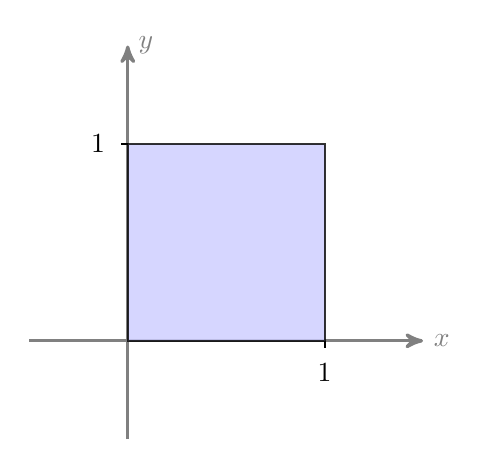
\begin{tikzpicture}[scale=2.5,
                          axis/.style={very thick, gray,->},
                          cube/.style={very thick, black},
                          mysolid/.style={very thick, black},
                          mydash/.style={thick, dashed, black},
                         ]


\coordinate (0) at (0,0);

\draw[axis] (-0.5,0) -- (1.5,0) node[right]{$x$};
\draw[axis] (0,-0.5) -- (0,1.5) node[right]{$y$};

\draw[thick, fill = blue!20!white, opacity=.8] (0,0) -- (1,0) -- (1,1) -- (0,1) -- cycle;

\draw[thick, black] (1,0) -- (1,-1pt) node[below,yshift=-2pt]{$1$};
\draw[thick, black] (0,1) -- (-1pt,1) node[left,xshift=-2pt]{$1$};

\end{tikzpicture}
\end{center}

\clearpage

\nin Our goal now is to manipulate this shape through linear transformations to make it look like something else.  The main geometric manipulations that we will be concerned with are

\begin{itemize}
\item translation
\item scaling
\item rotation
\item shearing
\end{itemize}

\vthree

\nin For now we will table the discussion of translation because it will throw a wrench into our whole operation.  The rest of the transformations can be done simply using $2 \times 2$ matrices operating on length-2 vectors that represent points.

\vthree

\nin {\bf Scaling}

\vspace{6mm}

\nin Consider the case when we want to scale the length of each of the side of the unit square until it looks like the following rectangle.

\vspace{10mm}

\begin{minipage}{.45\textwidth}
\begin{center}
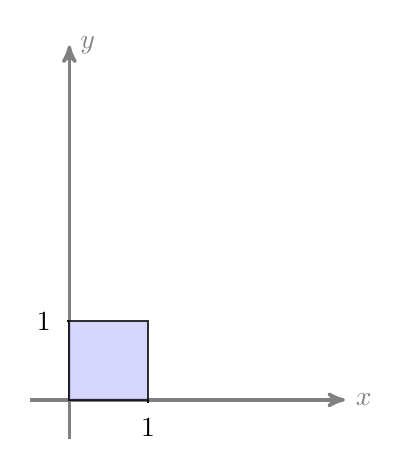
\begin{tikzpicture}[scale=1.0,
                          axis/.style={very thick, gray,->},
                          cube/.style={very thick, black},
                          mysolid/.style={very thick, black},
                          mydash/.style={thick, dashed, black},
                         ]


\coordinate (0) at (0,0);

\draw[axis] (-0.5,0) -- (3.5,0) node[right]{$x$};
\draw[axis] (0,-0.5) -- (0,4.5) node[right]{$y$};

\draw[thick, fill = blue!20!white, opacity=.8] (0,0) -- (1,0) -- (1,1) -- (0,1) -- cycle;

\draw[thick, black] (1,0) -- (1,-1pt) node[below,yshift=-2pt]{$1$};
\draw[thick, black] (0,1) -- (-1pt,1) node[left,xshift=-2pt]{$1$};

\end{tikzpicture}
\end{center}
\end{minipage}
\begin{minipage}{.1\textwidth}
\begin{center}
\[
\Huge\rightarrow\normalsize
\]
\end{center}
\end{minipage}
\begin{minipage}{.45\textwidth}
\begin{center}
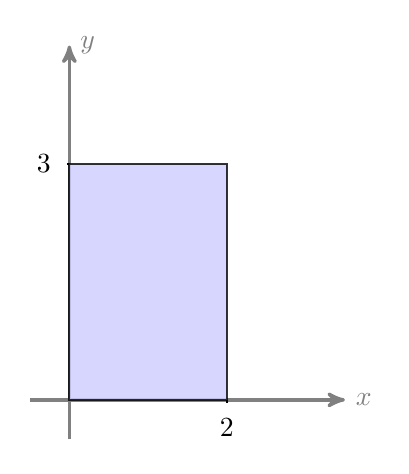
\begin{tikzpicture}[scale=1.0,
                          axis/.style={very thick, gray,->},
                          cube/.style={very thick, black},
                          mysolid/.style={very thick, black},
                          mydash/.style={thick, dashed, black},
                         ]


\coordinate (0) at (0,0);

\draw[axis] (-0.5,0) -- (3.5,0) node[right]{$x$};
\draw[axis] (0,-0.5) -- (0,4.5) node[right]{$y$};

\draw[thick, fill = blue!20!white, opacity=.8] (0,0) -- (2,0) -- (2,3) -- (0,3) -- cycle;

\draw[thick, black] (2,0) -- (2,-1pt) node[below,yshift=-2pt]{$2$};
\draw[thick, black] (0,3) -- (-1pt,3) node[left,xshift=-2pt]{$3$};

\end{tikzpicture}
\end{center}
\end{minipage}

\vthree

\nin Our goal is to find a $2 \times 2$ matrix $\hat{S}$ that transforms each of the vectors representing the vertices in the square into the corresponding vectors representing the vertices of the rectangle.

\vthree

\nin Note that one way to accomplish this is to choose $\hat{S}$ such that it scales a vector pointing in the $x$-direction to be twice its original length, and at the same time scales a vector pointing in the $y$-direction to be three times its original length.  To do this we can choose $\hat{S}$ so that it has the desired effect on the canonical basis vectors pointing in the $x$- and $y$-directions.

\vspace{10mm}

\begin{minipage}{.45\textwidth}
\begin{center}
\begin{tikzpicture}[scale=1.0,
                          axis/.style={very thick, gray,->},
                          cube/.style={very thick, black},
                          mysolid/.style={very thick, black},
                          mydash/.style={thick, dashed, black},
                         ]


\coordinate (0) at (0,0);

\draw[axis] (-0.5,0) -- (3.5,0) node[right]{$x$};
\draw[axis] (0,-0.5) -- (0,4.5) node[right]{$y$};

\draw[very thick, black, ->] (0,0) -- (1,0) node[below,yshift=-2pt]{\small$\be_1$\normalsize};
\draw[very thick, black, ->] (0,0) -- (0,1) node[left,xshift=-2pt]{\small$\be_2$\normalsize};


\end{tikzpicture}
\end{center}
\end{minipage}
\begin{minipage}{.1\textwidth}
\begin{center}
\[
\Huge\rightarrow\normalsize
\]
\end{center}
\end{minipage}
\begin{minipage}{.45\textwidth}
\begin{center}
\begin{tikzpicture}[scale=1.0,
                          axis/.style={very thick, gray,->},
                          cube/.style={very thick, black},
                          mysolid/.style={very thick, black},
                          mydash/.style={thick, dashed, black},
                         ]


\coordinate (0) at (0,0);

\draw[axis] (-0.5,0) -- (3.5,0) node[right]{$x$};
\draw[axis] (0,-0.5) -- (0,4.5) node[right]{$y$};

\draw[very thick, black, ->] (0,0) -- (2,0) node[below,yshift=-2pt,xshift=3pt]{\small$\hat{S}\be_1 = 2\be_1$\normalsize};
\draw[very thick, black, ->] (0,0) -- (0,3) node[left,xshift=-2pt]{\small$\hat{S}\be_2 = 3\be_2$\normalsize};


\end{tikzpicture}
\end{center}
\end{minipage}

\vthree

\nin The nice thing about operating on the the canonical basis vectors is that multiplication by $\hat{S}$ reveals the columns of $\hat{S}$.  Mathematically, we have


\[
\hat{S}\mymat{1 \\ 0} = \mymat{2 \\ 0}
\quad \quad \textrm{and} \quad \quad
\hat{S}\mymat{0 \\ 1} = \mymat{0 \\ 3}
\]

\vthree

\nin Since $\hat{S}\be_1$ should give us the first column of $\hat{S}$ and $\hat{S}\be_2$ should give us the second column of $\hat{S}$, we have

\[
\hat{S} =
\mymat{
2 & 0 \\
0 & 3
}
\]

\vthree

\nin To scale all of the vertices of the unit square at the same time, we can simply multiply the vertex matrix ${\bf X}$ by $\hat{S}$.  We have

\[
\hat{S}{\bf X} =
\mymat{
2 & 0 \\
0 & 3
}
\mymat{
0 & 1 & 1 & 0 \\
0 & 0 & 1 & 1 \\
}
=
\mymat{
0 & 2 & 2 & 0 \\
0 & 0 & 3 & 3 \\
}
\]

\vthree

\nin which are clearly the vertices of the desired rectangle.


\clearpage

\nin {\bf Rotations}

\vthree

\nin Consider now the case when we want to rotate the unit square some angle $\theta$ counterclockwise about the origin.  If we choose $\theta = \frac{\pi}{4}$ then the result looks as follows:

\vthree

\vspace{10mm}

\begin{minipage}{.45\textwidth}
\begin{center}
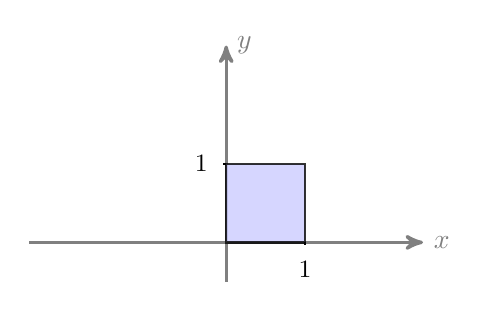
\begin{tikzpicture}[scale=1.0,
                          axis/.style={very thick, gray,->},
                          cube/.style={very thick, black},
                          mysolid/.style={very thick, black},
                          mydash/.style={thick, dashed, black},
                         ]


\coordinate (0) at (0,0);

\draw[axis] (-2.5,0) -- (2.5,0) node[right]{$x$};
\draw[axis] (0,-.5) -- (0,2.5) node[right]{$y$};

\draw[thick, fill = blue!20!white, opacity=.8] (0,0) -- (1,0) -- (1,1) -- (0,1) -- cycle;

\draw[thick, black] (1,0) -- (1,-1pt) node[below,yshift=-2pt]{\small$1$\normalsize};
\draw[thick, black] (0,1) -- (-1pt,1) node[left,xshift=-2pt]{\small$1$\normalsize};

\end{tikzpicture}
\end{center}
\end{minipage}
\begin{minipage}{.1\textwidth}
\begin{center}
\[
\Huge\rightarrow\normalsize
\]
\end{center}
\end{minipage}
\begin{minipage}{.45\textwidth}
\begin{center}
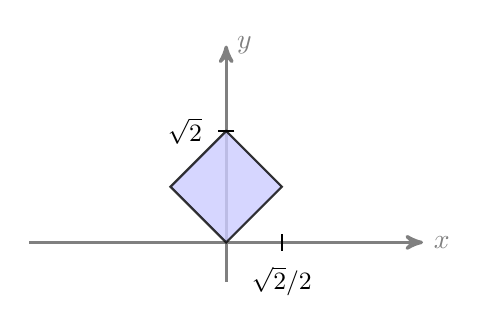
\begin{tikzpicture}[scale=1.0,
                          axis/.style={very thick, gray,->},
                          cube/.style={very thick, black},
                          mysolid/.style={very thick, black},
                          mydash/.style={thick, dashed, black},
                         ]


\coordinate (0) at (0,0);

\draw[axis] (-2.5,0) -- (2.5,0) node[right]{$x$};
\draw[axis] (0,-.5) -- (0,2.5) node[right]{$y$};

\draw[thick, fill = blue!20!white, opacity=.8] (0,0) -- ({sqrt(2)/2},{sqrt(2)/2}) -- (0,{sqrt(2)}) -- ({-sqrt(2)/2},{sqrt(2)/2}) -- cycle;

\draw[thick, black] (0.707,+3pt) -- (0.707,-3pt) node[below,yshift=-2pt]{\small$\sqrt{2}/2$\normalsize};
\draw[thick, black] (3pt,1.41) -- (-3pt,1.41) node[left,xshift=-2pt]{\small$\sqrt{2}$\normalsize};

\end{tikzpicture}
\end{center}
\end{minipage}

\vthree

\nin We can again accomplish this by choosing a matrix $\hat{R}$ that accomplishes the desired effect on the canonical basis vectors.  We'll figure out the rotation matrix for a genera $\theta$.  The desired effect on the basis vectors looks as follows



\begin{center}
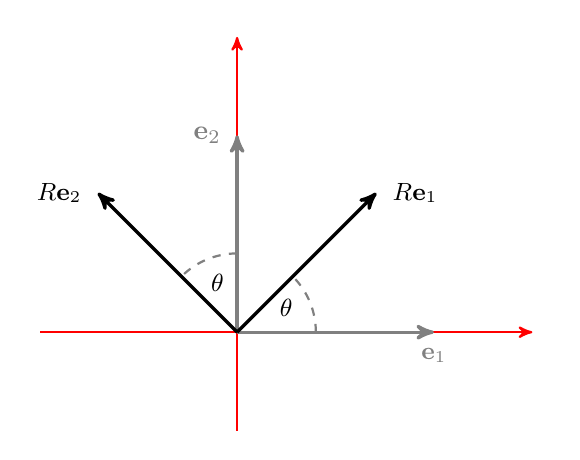
\begin{tikzpicture}[scale=2.5,
                          axis/.style={thick, red,->},
                          cube/.style={very thick, black},
                          mysolid/.style={very thick, black},
                          mydash/.style={thick, dashed, black},
                         ]


\coordinate (0) at (0,0);

\draw[axis] (-1,0) -- (1.5,0) node[right]{};
\draw[axis] (0,-.5) -- (0,1.5) node[right]{};

\draw[very thick, gray, ->] (0,0) -- (1,0) node[below,yshift=-2pt]{\small$\be_1$\normalsize};
\draw[very thick, gray, ->] (0,0) -- (0,1) node[left,xshift=-2pt]{$\be_2$};

\draw[very thick, black, ->] (0,0) -- ({sqrt(2)/2},{sqrt(2)/2}) node[right,xshift=2pt]{\small$R\be_1$\normalsize};
\draw[very thick, black, ->] (0,0) -- ({-sqrt(2)/2},{sqrt(2)/2}) node[left,xshift=-2pt]{\small$R\be_2$\normalsize};

\draw (.25,.125) node[]{\small$\theta$\normalsize};
\draw (-.1,.25) node[]{\small$\theta$\normalsize};

\draw[thick, dashed, gray, samples=100, domain=0:45] plot({.4*cos(\x)}, {.4*sin(\x)});
\draw[thick, dashed, gray, samples=100, domain=90:135] plot({.4*cos(\x)}, {.4*sin(\x)});

\end{tikzpicture}
\end{center}

\vthree

\nin A little trig convince us that we want $\hat{R}$ to have the following desired specific effect on $\be_1$ and $\be_2$:

\[
\hat{R}\mymat{1 \\ 0} =
\mymat{
\cos\theta \\
\sin\theta
}
\quad \quad \textrm{and}\quad\quad
\hat{R}\mymat{0 \\ 1} =
\mymat{
-\sin\theta \\
\cos\theta
}
\]

\vthree

\nin Thus the rotation matrix that rotates things $\theta$ radians about the origin is

\[
\hat{R} =
\mymat{
\cos\theta & -\sin\theta \\
\sin\theta & \cos\theta
}
\]

\vthree

\nin For the specific example with $\theta = \pi/4$ we have

\[
\hat{R} =
\mymat{
\sqrt{2}/2 & - \sqrt{2}/2 \\
\sqrt{2}/2 & \sqrt{2}/2 \\
}
\]

\clearpage

\nin Multiplying the coordinate matrix of the unit square by the rotation matrix gives the vertices of the rotated square:

\[
\hat{R}{\bf X} =
\mymat{
\sqrt{2}/2 & - \sqrt{2}/2 \\
\sqrt{2}/2 & \sqrt{2}/2 \\
}
\mymat{
0 & 1 & 1 & 0 \\
0 & 0 & 1 & 1 \\
} =
\mymat{
0 & \sqrt{2}/2 & 0 & -\sqrt{2} \\
0 & \sqrt{2}/2 & \sqrt{2} & \sqrt{2} \\
}
\]

\vthree

\nin which are of course the vertices  that we expect from the picture.

\vthree

\nin {\bf Shears}

\vthree

\nin Shear transformations allow us to turn squares into things like parallelogram.  There are shears in the horizontal direction and the vertical direction.  Application of a horizontal shear moves points in a horizontal direction proportional to their distance from the $x$-axis.  Consider the following shear transformation applied to the unit square in the first quadrant:

\vspace{10mm}

\begin{minipage}{.45\textwidth}
\begin{center}
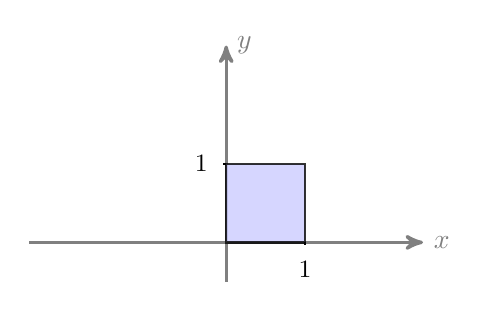
\begin{tikzpicture}[scale=1.0,
                          axis/.style={very thick, gray,->},
                          cube/.style={very thick, black},
                          mysolid/.style={very thick, black},
                          mydash/.style={thick, dashed, black},
                         ]


\coordinate (0) at (0,0);

\draw[axis] (-2.5,0) -- (2.5,0) node[right]{$x$};
\draw[axis] (0,-.5) -- (0,2.5) node[right]{$y$};

\draw[thick, fill = blue!20!white, opacity=.8] (0,0) -- (1,0) -- (1,1) -- (0,1) -- cycle;

\draw[thick, black] (1,0) -- (1,-1pt) node[below,yshift=-2pt]{\small$1$\normalsize};
\draw[thick, black] (0,1) -- (-1pt,1) node[left,xshift=-2pt]{\small$1$\normalsize};

\end{tikzpicture}
\end{center}
\end{minipage}
\begin{minipage}{.1\textwidth}
\begin{center}
\[
\Huge\rightarrow\normalsize
\]
\end{center}
\end{minipage}
\begin{minipage}{.45\textwidth}
\begin{center}
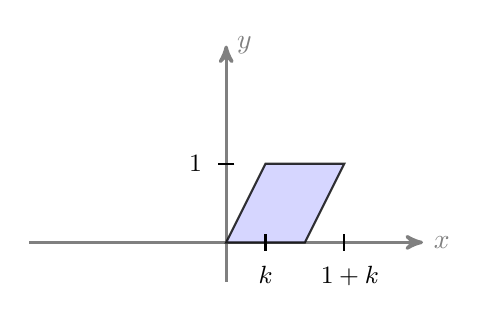
\begin{tikzpicture}[scale=1.0,
                          axis/.style={very thick, gray,->},
                          cube/.style={very thick, black},
                          mysolid/.style={very thick, black},
                          mydash/.style={thick, dashed, black},
                         ]


\coordinate (0) at (0,0);

\draw[axis] (-2.5,0) -- (2.5,0) node[right]{$x$};
\draw[axis] (0,-.5) -- (0,2.5) node[right]{$y$};

\draw[thick, fill = blue!20!white, opacity=.8] (0,0) -- (1,0) -- (1.5, 1) -- (.5, 1) -- cycle;

% \draw[thick, black] (1,3pt) -- (1,-3pt) node[below,yshift=-2pt]{\small$1$\normalsize};
\draw[thick, black] (.5,3pt) -- (.5,-3pt) node[below,yshift=-2pt]{\small$k$\normalsize};
\draw[thick, black] (1.5,3pt) -- (1.5,-3pt) node[below,yshift=-2pt,xshift=2pt]{\small$1+k$\normalsize};
\draw[thick, black] (3pt,1) -- (-3pt,1) node[left,xshift=-2pt]{\small$1$\normalsize};

\end{tikzpicture}
\end{center}
\end{minipage}

\vthree

\nin The shear transformation pictured here moved the vertices lying on the line $y=1$ to the right $k$ units.  To determine the matrix $\hat{H}$ that applies this transformation we again consider how the transformation moves the first two canonical basis vectors.

\vspace{10mm}

\begin{center}
\begin{tikzpicture}[scale=2.5,
                          axis/.style={thick, red,->},
                          cube/.style={very thick, black},
                          mysolid/.style={very thick, black},
                          mydash/.style={thick, dashed, black},
                         ]


\coordinate (0) at (0,0);

\draw[axis] (-1,0) -- (1.5,0) node[right]{};
\draw[axis] (0,-.5) -- (0,1.5) node[right]{};

\draw[very thick, gray, ->] (0,0) -- (0,1) node[left,xshift=-2pt]{\small$\be_2$\normalsize};

\draw[very thick, black, ->] (0,0) -- (1,0) node[below,xshift=2pt]{\small$\hat{H}\be_1 = \be_1$\normalsize};
\draw[very thick, black, ->] (0,0) -- (0.5,1) node[right,xshift=-2pt]{\small$\hat{H}\be_2 = k\be_1 + \be_2$\normalsize};

\end{tikzpicture}
\end{center}

\vthree

\nin From this we see that

\[
\hat{H}\mymat{1 \\ 0} = \mymat{1 \\ 0}
\quad \textrm{and} \quad
\hat{H}\mymat{0 \\ 1} = \mymat{k \\ 1}
\]

\clearpage

\nin Thus the horizontal shear matrix is given by

\[
\hat{H} =
\mymat{
1 & k \\
0 & 1
}
\]

\vthree

\nin A similar analysis shows that the vertical shearing matrix $\hat{V} = \mymat{1 & 0 \\ k & 1}$ performs the following transformation

\vspace{10mm}

\begin{minipage}{.45\textwidth}
\begin{center}
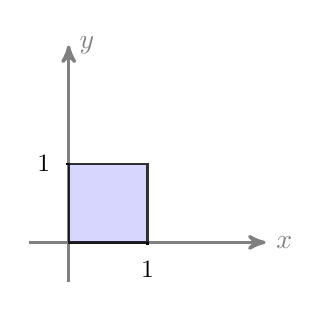
\begin{tikzpicture}[scale=1.0,
                          axis/.style={very thick, gray,->},
                          cube/.style={very thick, black},
                          mysolid/.style={very thick, black},
                          mydash/.style={thick, dashed, black},
                         ]


\coordinate (0) at (0,0);

\draw[axis] (-.5,0) -- (2.5,0) node[right]{$x$};
\draw[axis] (0,-.5) -- (0,2.5) node[right]{$y$};

\draw[thick, fill = blue!20!white, opacity=.8] (0,0) -- (1,0) -- (1,1) -- (0,1) -- cycle;

\draw[thick, black] (1,0) -- (1,-1pt) node[below,yshift=-2pt]{\small$1$\normalsize};
\draw[thick, black] (0,1) -- (-1pt,1) node[left,xshift=-2pt]{\small$1$\normalsize};

\end{tikzpicture}
\end{center}
\end{minipage}
\begin{minipage}{.1\textwidth}
\begin{center}
\[
\Huge\rightarrow\normalsize
\]
\end{center}
\end{minipage}
\begin{minipage}{.45\textwidth}
\begin{center}
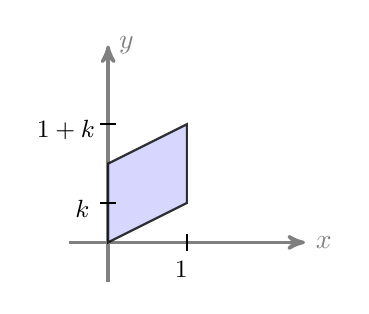
\begin{tikzpicture}[scale=1.0,
                          axis/.style={very thick, gray,->},
                          cube/.style={very thick, black},
                          mysolid/.style={very thick, black},
                          mydash/.style={thick, dashed, black},
                         ]


\coordinate (0) at (0,0);

\draw[axis] (-.5,0) -- (2.5,0) node[right]{$x$};
\draw[axis] (0,-.5) -- (0,2.5) node[right]{$y$};

\draw[thick, fill = blue!20!white, opacity=.8] (0,0) -- (1,0.5) -- (1, 1.5) -- (0, 1) -- cycle;

% \draw[thick, black] (1,3pt) -- (1,-3pt) node[below,yshift=-2pt]{\small$1$\normalsize};
\draw[thick, black] (1,3pt) -- (1,-3pt) node[below,xshift=-2pt]{\small$1$\normalsize};
\draw[thick, black] (3pt,.5) -- (-3pt,.5) node[left,yshift=-2pt]{\small$k$\normalsize};
\draw[thick, black] (3pt, 1.5) -- (-3pt,1.5) node[left,yshift=-2pt,xshift=2pt]{\small$1+k$\normalsize};

\end{tikzpicture}
\end{center}
\end{minipage}

\vthree

\nin {\bf Translation}

\vthree

\nin Translation is the transformation that moves an object a fixed distance in the $x$ and $y$-directions.  In the image below the unit square is translated $x_0$ in the $x$-direction and $y_0$ in the $y$-direction.

\vspace{10mm}

\begin{minipage}{.45\textwidth}
\begin{center}
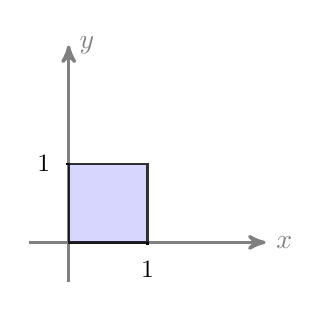
\begin{tikzpicture}[scale=1.0,
                          axis/.style={very thick, gray,->},
                          cube/.style={very thick, black},
                          mysolid/.style={very thick, black},
                          mydash/.style={thick, dashed, black},
                         ]


\coordinate (0) at (0,0);

\draw[axis] (-.5,0) -- (2.5,0) node[right]{$x$};
\draw[axis] (0,-.5) -- (0,2.5) node[right]{$y$};

\draw[thick, fill = blue!20!white, opacity=.8] (0,0) -- (1,0) -- (1,1) -- (0,1) -- cycle;

\draw[thick, black] (1,0) -- (1,-1pt) node[below,yshift=-2pt]{\small$1$\normalsize};
\draw[thick, black] (0,1) -- (-1pt,1) node[left,xshift=-2pt]{\small$1$\normalsize};

\end{tikzpicture}
\end{center}
\end{minipage}
\begin{minipage}{.1\textwidth}
\begin{center}
\[
\Huge\rightarrow\normalsize
\]
\end{center}
\end{minipage}
\begin{minipage}{.45\textwidth}
\begin{center}
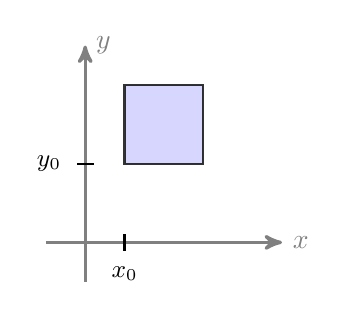
\begin{tikzpicture}[scale=1.0,
                          axis/.style={very thick, gray,->},
                          cube/.style={very thick, black},
                          mysolid/.style={very thick, black},
                          mydash/.style={thick, dashed, black},
                         ]


\coordinate (0) at (0,0);

\draw[axis] (-.5,0) -- (2.5,0) node[right]{$x$};
\draw[axis] (0,-.5) -- (0,2.5) node[right]{$y$};

\draw[thick, fill = blue!20!white, opacity=.8] (0.5,1) -- (1.5,1) -- (1.5,2) -- (0.5,2) -- cycle;

\draw[thick, black] (0.5,3pt) -- (0.5,-3pt) node[below,yshift=-2pt]{\small$x_0$\normalsize};
\draw[thick, black] (3pt,1) -- (-3pt,1) node[left,xshift=-2pt]{\small$y_0$\normalsize};

\end{tikzpicture}
\end{center}
\end{minipage}

\vthree

\nin Unfortunately, we cannot find a matrix $T$ that performs the translation operation, because translation is not a linear operation.  To see this, recognize that there is no matrix that can transform the origin (i.e. the zero vector) into a nonzero vector.  To overcome this we have to increase the dimension of the space that we're working in.

\vthree

\nin Instead of representing the point $\myp{x,y}$ by the vector $\mymat{x \\ y}$ we represent it by $\mymat{x \\ y \\ 1}$.

\vthree

\nin The extra $1$ in the third entry will allow us to perform translations by multiplication by a $3 \times 3$ matrix.  The representation of $\myp{x,y}$ by the length-3 vectors is called the {\it homogeneous coordinate system}.  For our purposes, the third coordinate will always be a $1$, but there are interpretations of the coordinate system where it can take on different values.

\clearpage

\nin OK, so how to we represent the above transformation by a $3 \times 3$ matrix?  Our goal is to find a matrix $T$ such that

\[
T \mymat{x \\ y \\ 1} = \mymat{x + x_0 \\ y + y_0 \\ 1}
\]

\vthree

\nin Interpreting multiplication by $T$ as a linear combination of its columns, we have

\[
T \mymat{x \\ y \\ 1} =
x\mymat{\phantom{x} \\ \phantom{x} \\ \phantom{x}} +
y\mymat{\phantom{x} \\ \phantom{x} \\ \phantom{x}} +
1\mymat{\phantom{x} \\ \phantom{x} \\ \phantom{x}}
=
\mymat{x + x_0 \\ y + y_0 \\ 1}
\]

\vthree

\nin Filling in the entries of the column vectors to put the appropriate values of $x$, $y$, $x_0$, and $y_0$ in the correct positions, we have

\vthree

\[
T \mymat{x \\ y \\ 1} =
x\mymat{1 \\ 0 \\ 0} +
y\mymat{0 \\ 1 \\ 0} +
1\mymat{x_0 \\ y_0 \\ 1}
=
\mymat{x + x_0 \\ y + y_0 \\ 1}
\]

\vthree

\nin which gives us the translation matrix $T =
\mymat{
 1 & 0 & x_0 \\
 0 & 1 & y_0 \\
 0 & 0 & 1 \\
}
$

\vthree

\nin Now, we want to use a consistent coordinate system that allows us to perform scalings, rotations, shears, and translations.  Because of the translations, we'll use the homogeneous coordinate systems for them all.  This means that we need to come up with $3 \times 3$ representations of the non-translation transformations.  This turns out to be fairly simple.  We simply replace each transformation by a $3 \times 3$ identity and replace it's upper $2 \times 2$ block with the desired $2 \times 2$ transformation matrix.

\vthree

\[
S =
\mymat{
c_1 & 0 & 0 \\
0 & c_2 & 0 \\
0 & 0 & 1 \\
}
\quad \quad
R =
\mymat{
\cos\theta & -\sin\theta & 0 \\
\sin\theta & \cos\theta & 0 \\
0 & 0 & 1 \\
}
\quad \quad
H =
\mymat{
1 & k & 0 \\
0 & 1 & 0 \\
0 & 0 & 1 \\
}
\]

\vthree

\nin Note that since the last row and column of each matrix have only a $1$ in the $(3,3)$-position, the third entry of the homogeneous coordinate vector does not affect the action of the original transformation.

\clearpage

\nin {\bf Composite Transformations}

\vthree

\nin Most interesting shapes are created by applying multiply simple transformations to a representative shape, like the unit square.

\vthree

\nin {\bf Example 1}: Suppose that we want to transform the unit square into the following shape:

\vspace{10mm}

\begin{center}
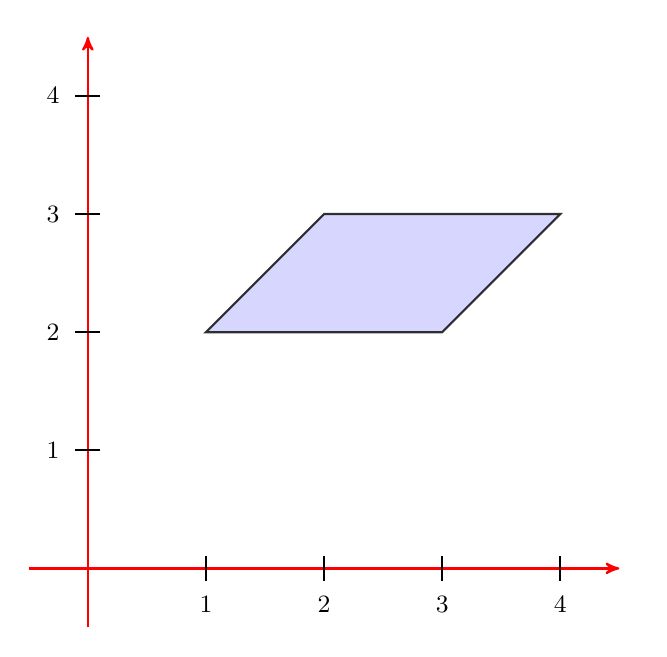
\begin{tikzpicture}[scale=1.5,
                          axis/.style={thick, red,->},
                          cube/.style={very thick, black},
                          mysolid/.style={very thick, black},
                          mydash/.style={thick, dashed, black},
                         ]


\coordinate (0) at (0,0);

\draw[axis] (-.5,0) -- (4.5,0) node[right]{};
\draw[axis] (0,-.5) -- (0,4.5) node[right]{};

\draw[thick, fill = blue!20!white, opacity=.8] (1,2) -- (3,2) -- (4,3) -- (2,3) -- cycle;

\draw[thick, black] (1,3pt) -- (1,-3pt) node[below,yshift=-2pt]{\small$1$\normalsize};
\draw[thick, black] (2,3pt) -- (2,-3pt) node[below,yshift=-2pt]{\small$2$\normalsize};
\draw[thick, black] (3,3pt) -- (3,-3pt) node[below,yshift=-2pt]{\small$3$\normalsize};
\draw[thick, black] (4,3pt) -- (4,-3pt) node[below,yshift=-2pt]{\small$4$\normalsize};
\draw[thick, black] (3pt,1) -- (-3pt,1) node[left,xshift=-2pt]{\small$1$\normalsize};
\draw[thick, black] (3pt,2) -- (-3pt,2) node[left,xshift=-2pt]{\small$2$\normalsize};
\draw[thick, black] (3pt,3) -- (-3pt,3) node[left,xshift=-2pt]{\small$3$\normalsize};
\draw[thick, black] (3pt,4) -- (-3pt,4) node[left,xshift=-2pt]{\small$4$\normalsize};

\end{tikzpicture}
\end{center}

\vthree

\nin One way to accomplish this is

\ben
\item Scale the square to a rectangle two units wide and one unit tall.
\item Apply a horizontal shear with $k=1$
\item Translate the result two units in the $y$-direction and one unit in the $x$-direction.
\een

\vthree

\nin If we let ${\bf X}$ be the coordinate matrix describing the unit square, the new shape will be given by

\[
{\bf X}_{\textrm{new}} = THS \hs {\bf X}
\]

\vthree

\nin where

\vthree

\[
S =
\mymat{
2 & 0 & 0 \\
0 & 1 & 0 \\
0 & 0 & 1 \\
}
\quad \quad
H =
\mymat{
1 & 1 & 0 \\
0 & 1 & 0 \\
0 & 0 & 1 \\
}
\quad \quad
T =
\mymat{
1 & 0 & 1 \\
0 & 1 & 2 \\
0 & 0 & 1 \\
}
\]

\clearpage

\nin We have

\[
S{\bf X} =
\mymat{
2 & 0 & 0 \\
0 & 1 & 0 \\
0 & 0 & 1 \\
}
\mymat{
0 & 1 & 1 & 0 \\
0 & 0 & 1 & 1 \\
1 & 1 & 1 & 1 \\
}
=
\mymat{
0 & 2 & 2 & 0 \\
0 & 0 & 1 & 1 \\
1 & 1 & 1 & 1 \\
}
\]

\vthree

\[
H\myp{S{\bf X}} =
\mymat{
1 & 1 & 0 \\
0 & 1 & 0 \\
0 & 0 & 1 \\
}
\mymat{
0 & 2 & 2 & 0 \\
0 & 0 & 1 & 1 \\
1 & 1 & 1 & 1 \\
}
=
\mymat{
0 & 2 & 3 & 1 \\
0 & 0 & 1 & 1 \\
1 & 1 & 1 & 1 \\
}
\]

\vthree

\[
T\myp{HS{\bf X}} =
\mymat{
1 & 0 & 1 \\
0 & 1 & 2 \\
0 & 0 & 1 \\
}
\mymat{
0 & 2 & 3 & 1 \\
0 & 0 & 1 & 1 \\
1 & 1 & 1 & 1 \\
}
=
\mymat{
1 & 3 & 4 & 2 \\
2 & 2 & 3 & 3 \\
1 & 1 & 1 & 1 \\
}
\]

\vthree

\nin Notice that the first two entries of the four column-vectors of ${\bf X}$ are the precise coordinates of the parallelogram in the example.

\vthree

\nin {\bf Example 2}: Suppose that we want to take a cube of side length 2 centered at the point $\myp{2,2}$ and rotate it $\pi/4$ radians counterclockwise about it's center.

\vspace{10mm}

\begin{minipage}{.45\textwidth}
\begin{center}
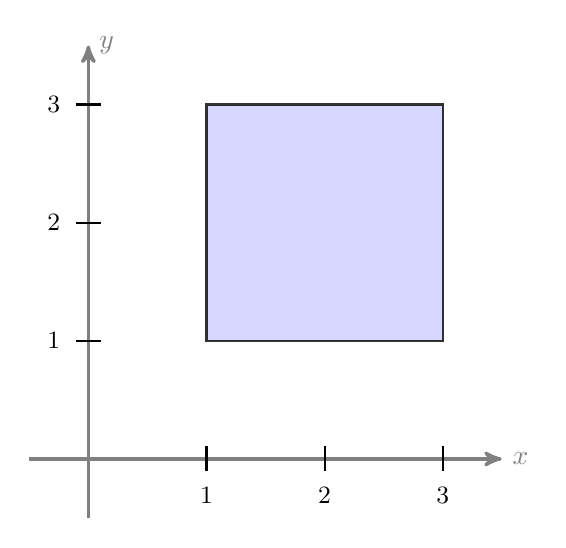
\begin{tikzpicture}[scale=1.5,
                          axis/.style={very thick, gray,->},
                          cube/.style={very thick, black},
                          mysolid/.style={very thick, black},
                          mydash/.style={thick, dashed, black},
                         ]


\coordinate (0) at (0,0);

\draw[axis] (-.5,0) -- (3.5,0) node[right]{$x$};
\draw[axis] (0,-.5) -- (0,3.5) node[right]{$y$};

\draw[thick, fill = blue!20!white, opacity=.8] (1,1) -- (3,1) -- (3,3) -- (1,3) -- cycle;

\draw[thick, black] (1,3pt) -- (1,-3pt) node[below,yshift=-2pt]{\small$1$\normalsize};
\draw[thick, black] (2,3pt) -- (2,-3pt) node[below,yshift=-2pt]{\small$2$\normalsize};
\draw[thick, black] (3,3pt) -- (3,-3pt) node[below,yshift=-2pt]{\small$3$\normalsize};
\draw[thick, black] (3pt,1) -- (-3pt,1) node[left,xshift=-2pt]{\small$1$\normalsize};
\draw[thick, black] (3pt,2) -- (-3pt,2) node[left,xshift=-2pt]{\small$2$\normalsize};
\draw[thick, black] (3pt,3) -- (-3pt,3) node[left,xshift=-2pt]{\small$3$\normalsize};

\end{tikzpicture}
\end{center}
\end{minipage}
\begin{minipage}{.1\textwidth}
\begin{center}
\[
\Huge\rightarrow\normalsize
\]
\end{center}
\end{minipage}
\begin{minipage}{.45\textwidth}
\begin{center}
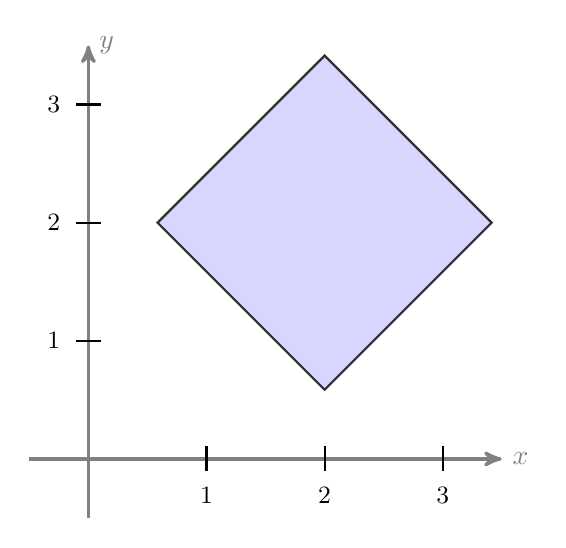
\begin{tikzpicture}[scale=1.5,
                          axis/.style={very thick, gray,->},
                          cube/.style={very thick, black},
                          mysolid/.style={very thick, black},
                          mydash/.style={thick, dashed, black},
                         ]


\coordinate (0) at (0,0);

\draw[axis] (-.5,0) -- (3.5,0) node[right]{$x$};
\draw[axis] (0,-.5) -- (0,3.5) node[right]{$y$};

\draw[thick, fill = blue!20!white, opacity=.8] (2.0,.5858) -- (3.41421,2.0) -- (2.0,3.41421) -- (0.5858,2.0) -- cycle;


\draw[thick, black] (1,3pt) -- (1,-3pt) node[below,yshift=-2pt]{\small$1$\normalsize};
\draw[thick, black] (2,3pt) -- (2,-3pt) node[below,yshift=-2pt]{\small$2$\normalsize};
\draw[thick, black] (3,3pt) -- (3,-3pt) node[below,yshift=-2pt]{\small$3$\normalsize};
\draw[thick, black] (3pt,1) -- (-3pt,1) node[left,xshift=-2pt]{\small$1$\normalsize};
\draw[thick, black] (3pt,2) -- (-3pt,2) node[left,xshift=-2pt]{\small$2$\normalsize};
\draw[thick, black] (3pt,3) -- (-3pt,3) node[left,xshift=-2pt]{\small$3$\normalsize};


\end{tikzpicture}
\end{center}
\end{minipage}

\vthree

\nin Recall that the simple rotation transformation rotates points about the origin.  This means that we cannot accomplish this transformation with a simple rotation.  Since we want to rotate the square about the point $(2,2)$ our strategy will be to translate the square so that the point $(2,2)$ moves to the origin, rotate the square about the origin, and translate it back to it's original position.

\clearpage

\nin This can be accomplished by the following composition of simple transformations

\[
{\bf X}_{\textrm{new}} = T_2 \hs R \hs T_1 \hs {\bf X}
\]

\nin where

\[
T_1 =
\mymat{
1 & 0 &-2 \\
0 & 1 &-2 \\
0 & 0 & 1 \\
}
\quad \quad
R =
\mymat{
\sqrt{2}/2 & -\sqrt{2}/2 & 0 \\
\sqrt{2}/2 & \sqrt{2}/2 & 0 \\
0 & 0 & 1 \\
}
\quad \quad
T_2 =
\mymat{
1 & 0 & 2 \\
0 & 1 & 2 \\
0 & 0 & 1 \\
}
\]

\vthree

\nin The homogeneous coordinates of the original square are given by

\[
{\bf X} =
\mymat{
1 & 3 & 3 & 1 \\
1 & 1 & 3 & 3 \\
1 & 1 & 1 & 1 \\
}
\]

\vthree

\nin We then have

\[
T_1 {\bf X} =
\mymat{
1 & 0 &-2 \\
0 & 1 &-2 \\
0 & 0 & 1 \\
}
\mymat{
1 & 3 & 3 & 1 \\
1 & 1 & 3 & 3 \\
1 & 1 & 1 & 1 \\
}
=
\mymat{
-1 & 1 & 1 &-1 \\
-1 &-1 & 1 & 1 \\
1  & 1 & 1 & 1 \\
}
\]

\vthree

\[
R\myp{T_1 {\bf X}} =
\mymat{
\sqrt{2}/2 & -\sqrt{2}/2 & 0 \\
\sqrt{2}/2 & \sqrt{2}/2 & 0 \\
0 & 0 & 1 \\
}
\mymat{
-1 & 1 & 1 &-1 \\
-1 &-1 & 1 & 1 \\
1  & 1 & 1 & 1 \\
}
=
\mymat{
0         & \sqrt{2} & 0        &-\sqrt{2} \\
-\sqrt{2} & 0        & \sqrt{2} & 0 \\
1  & 1 & 1 & 1 \\
}
\]

\vthree

\[
T_2\myp{RT_1 {\bf X}} =
\mymat{
1 & 0 & 2 \\
0 & 1 & 2 \\
0 & 0 & 1 \\
}
\mymat{
0         & \sqrt{2} & 0        &-\sqrt{2} \\
-\sqrt{2} & 0        & \sqrt{2} & 0 \\
1  & 1 & 1 & 1 \\
}
=
\mymat{
2         & 2+\sqrt{2} & 2        &2-\sqrt{2} \\
2-\sqrt{2} & 2        & 2+\sqrt{2} & 2 \\
1  & 1 & 1 & 1 \\
}
\]

\vthree

\nin The extension of these transformations to three dimensions is relatively straight forward.  We will only consider scalings, rotations, and translations.  Of these the only one that is not identical to its 2D transformation is rotation.

\vthree

\nin A point in three dimensions $\myp{x,y,z}$ is represented in homogeneous coordinates by a four dimensional vector with the fourth entry equal to $1$:


\[
\myp{x,y,z} \quad \mapsto \quad \mymat{x \\ y \\ z \\ 1}
\]

\clearpage

\nin Scaling an object in three dimensions by $c_1$ in the $x$-direction, $c_2$ in the $y$-direction, and $c_3$ in the $z$-direction is given by the diagonal matrix

\[
S =
\mymat{
c_1 & 0 & 0     & 0 \\
0   & c_2 & 0   & 0 \\
0   & 0   & c_3 & 0 \\
0   & 0   & 0   & 1 \\
}
\]

\vthree

\nin Translation of a point a fixed amount in each coordinate direction is analogous to it's 2D variant.  The transformation

\[
\myp{x,y,z} \quad \mapsto \quad \myp{x+x_0, y+y_0, z+z_0}
\]

\nin is given by the matrix

\[
T =
\mymat{
1 & 0 & 0 & x_0 \\
0 & 1 & 0 & y_0 \\
0 & 0 & 1 & z_0 \\
0 & 0 & 0 & 1 \\
}
\]

\vthree

\nin Rotations pose a slight complication.  It no longer makes sense to talk about a rotation about the origin since this is inherently ambiguous.  Instead we can build rotations based on simple rotations about each of the coordinate axes.  For example, the 2D rotation of vectors in the $xy$-plane considered before can be interpreted as rotation about the $z$-axis.  Rotation an angle $\theta$ in the counterclockwise direction is depicted below.


\vspace{10mm}

\begin{minipage}{.45\textwidth}
\begin{center}
\begin{tikzpicture}[scale=2.5,
              tdplot_main_coords,
              axis/.style={thick, red,->},
              cube/.style={very thick, black},
              mydash/.style={thick, dashed, black},
             ]

\coordinate (0) at (0,0,0);

\draw[axis] (0,0,0) -- (1.5,0,0) node[anchor=north east]{$x$};
\draw[axis] (0,0,0) -- (0,1.5,0) node[anchor=north west]{$y$};
\draw[axis] (0,0,0) -- (0,0,1.5) node[anchor=south]{$z$};

\draw[very thick,->] (0,0,0) -- (1,0,0) node[above,yshift=3pt]{$\be_1$};
\draw[very thick,->] (0,0,0) -- (0,1,0) node[above,yshift=2pt]{$\be_2$};
\draw[very thick,->] (0,0,0) -- (0,0,1) node[left,xshift=2pt]{$\be_3$};

\end{tikzpicture}
\end{center}
\end{minipage}
\begin{minipage}{.1\textwidth}
\begin{center}
\[
\Huge\rightarrow\normalsize
\]
\end{center}
\end{minipage}
\begin{minipage}{.45\textwidth}
\begin{center}
\begin{tikzpicture}[scale=2.5,
              tdplot_main_coords,
              axis/.style={thick, red,->},
              cube/.style={very thick, black},
              mydash/.style={thick, dashed, black},
             ]

\coordinate (0) at (0,0,0);

\draw[axis] (0,0,0) -- (1.5,0,0) node[anchor=north east]{$x$};
\draw[axis] (0,0,0) -- (0,1.5,0) node[anchor=north west]{$y$};
\draw[axis] (0,0,0) -- (0,0,1.5) node[anchor=south]{$z$};

\draw[very thick,->] (0,0,0) -- ({ cos(20)}, { sin(20)},0) node[below,yshift=3pt]{$\hat{R}_z\be_1$};
\draw[very thick,->] (0,0,0) -- ({-sin(20)}, { cos(20)},0) node[above,yshift=2pt]{$\hat{R}_z\be_2$};
\draw[very thick,->] (0,0,0) -- (0,0,1) node[left,xshift=2pt]{$\hat{R}_z\be_3$};

\draw (.5,.10, 0) node[]{$\tiny \theta \normalsize$};

\end{tikzpicture}
\end{center}
\end{minipage}

\vthree

\nin From the picture and a little trig we see that the canonical basis vectors transform as follows

\[
\hat{R}_z\mymat{
1 \\
0 \\
0
}
=
\mymat{
\cos\theta \\
\sin\theta \\
0 \\
}
\quad
\hat{R}_z\mymat{
0 \\
1 \\
0
}
=
\mymat{
-\sin\theta \\
\cos\theta \\
0 \\
}
\quad
\hat{R}_z\mymat{
0 \\
0 \\
1
}
=
\mymat{
0 \\
0 \\
1 \\
}
\]

\clearpage

\nin Adding the identity row and column corresponding to the homogeneous coordinate we have

\[
R_z =
\mymat{
\cos\theta & -\sin\theta & 0 & 0 \\
\sin\theta &  \cos\theta & 0 & 0 \\
0 & 0 & 1 & 0 \\
0 & 0 & 0 & 1 \\
}
\]

\vthree

\nin Rotation about the $x$-axis is similar.  The picture looks like

\vspace{10mm}

\begin{minipage}{.45\textwidth}
\begin{center}
\begin{tikzpicture}[scale=2.5,
              tdplot_main_coords,
              axis/.style={thick, red,->},
              cube/.style={very thick, black},
              mydash/.style={thick, dashed, black},
             ]

\coordinate (0) at (0,0,0);

\draw[axis] (0,0,0) -- (1.5,0,0) node[anchor=north east]{$x$};
\draw[axis] (0,0,0) -- (0,1.5,0) node[anchor=north west]{$y$};
\draw[axis] (0,0,0) -- (0,0,1.5) node[anchor=south]{$z$};

\draw[very thick,->] (0,0,0) -- (1,0,0) node[above,yshift=3pt]{$\be_1$};
\draw[very thick,->] (0,0,0) -- (0,1,0) node[above,yshift=2pt]{$\be_2$};
\draw[very thick,->] (0,0,0) -- (0,0,1) node[left,xshift=2pt]{$\be_3$};

\end{tikzpicture}
\end{center}
\end{minipage}
\begin{minipage}{.1\textwidth}
\begin{center}
\[
\Huge\rightarrow\normalsize
\]
\end{center}
\end{minipage}
\begin{minipage}{.45\textwidth}
\begin{center}
\begin{tikzpicture}[scale=2.5,
              tdplot_main_coords,
              axis/.style={thick, red,->},
              cube/.style={very thick, black},
              mydash/.style={thick, dashed, black},
             ]

\coordinate (0) at (0,0,0);

\draw[axis] (0,0,0) -- (1.5,0,0) node[anchor=north east]{$x$};
\draw[axis] (0,0,0) -- (0,1.5,0) node[anchor=north west]{$y$};
\draw[axis] (0,0,0) -- (0,0,1.5) node[anchor=south]{$z$};

\draw[very thick,->] (0,0,0) -- (0, {-sin(20)}, { cos(20)}) node[above,yshift=2pt]{$\hat{R}_x\be_3$};
\draw[very thick,->] (0,0,0) -- (0, { cos(20)}, { sin(20)}) node[above,yshift=2pt]{$\hat{R}_x\be_2$};
\draw[very thick,->] (0,0,0) -- (1,0,0) node[left,xshift=0pt,yshift=4pt]{$\hat{R}_x\be_1$};

\draw (0,-.07,.5,) node[]{$\tiny \theta \normalsize$};

\end{tikzpicture}
\end{center}
\end{minipage}

\vthree

\nin We have

\[
\hat{R}_x\mymat{
1 \\
0 \\
0
}
=
\mymat{
1 \\
0 \\
0 \\
}
\quad
\hat{R}_x\mymat{
0 \\
1 \\
0
}
=
\mymat{
0 \\
\cos\theta \\
\sin\theta \\
}
\quad
\hat{R}_x\mymat{
0 \\
0 \\
1
}
=
\mymat{
0 \\
-\sin\theta \\
\cos\theta \\
}
\]

\vthree

\nin The transformation matrix in the homogeneous coordinate system is given by

\[
R_x =
\mymat{
1 & 0 & 0 & 0 \\
0 & \cos\theta & -\sin\theta  & 0 \\
0 & \sin\theta &  \cos\theta  & 0 \\
0 & 0 & 0 & 1 \\
}
\]

\vthree

\nin Note that the $x$-axis rotation matrix looks very similar to the $z$-axis rotation matrix but with the roles of $x$ and $y$ replaced by $y$ and $z$.  Rotation about the $y$-axis is a slightly different animal.  The picture looks as follows

\vspace{10mm}

\begin{minipage}{.45\textwidth}
\begin{center}
\begin{tikzpicture}[scale=2.5,
              tdplot_main_coords,
              axis/.style={thick, red,->},
              cube/.style={very thick, black},
              mydash/.style={thick, dashed, black},
             ]

\coordinate (0) at (0,0,0);

\draw[axis] (0,0,0) -- (1.5,0,0) node[anchor=north east]{$x$};
\draw[axis] (0,0,0) -- (0,1.5,0) node[anchor=north west]{$y$};
\draw[axis] (0,0,0) -- (0,0,1.5) node[anchor=south]{$z$};

\draw[very thick,->] (0,0,0) -- (1,0,0) node[above,yshift=3pt]{$\be_1$};
\draw[very thick,->] (0,0,0) -- (0,1,0) node[above,yshift=2pt]{$\be_2$};
\draw[very thick,->] (0,0,0) -- (0,0,1) node[left,xshift=2pt]{$\be_3$};

\end{tikzpicture}
\end{center}
\end{minipage}
\begin{minipage}{.1\textwidth}
\begin{center}
\[
\Huge\rightarrow\normalsize
\]
\end{center}
\end{minipage}
\begin{minipage}{.45\textwidth}
\begin{center}
\begin{tikzpicture}[scale=2.5,
              tdplot_main_coords,
              axis/.style={thick, red,->},
              cube/.style={very thick, black},
              mydash/.style={thick, dashed, black},
             ]

\coordinate (0) at (0,0,0);

\draw[axis] (0,0,0) -- (1.5,0,0) node[anchor=north east]{$x$};
\draw[axis] (0,0,0) -- (0,1.5,0) node[anchor=north west]{$y$};
\draw[axis] (0,0,0) -- (0,0,1.5) node[anchor=south]{$z$};

\draw[very thick,->] (0,0,0) -- (0,1,0) node[above,xshift=0pt,yshift=4pt]{$\hat{R}_y\be_2$};
\draw[very thick,->] (0,0,0) -- ({ sin(20)}, 0, { cos(20)}) node[above,xshift=-2pt]{$\hat{R}_y\be_3$};
\draw[very thick,->] (0,0,0) -- ({ cos(20)}, 0, {-sin(20)}) node[below,yshift=-2pt]{$\hat{R}_y\be_1$};

\draw (0,-.07,.55,) node[]{$\tiny \theta \normalsize$};

\end{tikzpicture}
\end{center}
\end{minipage}

\vthree

\nin We have

\[
\hat{R}_y\mymat{
1 \\
0 \\
0
}
=
\mymat{
\cos\theta \\
0 \\
-\sin\theta \\
}
\quad
\hat{R}_y\mymat{
0 \\
1 \\
0
}
=
\mymat{
0 \\
1 \\
0
}
\quad
\hat{R}_y\mymat{
0 \\
0 \\
1
}
=
\mymat{
\sin\theta \\
1 \\
\cos\theta \\
}
\]

\vthree

\nin The transformation matrix in homogeneous coordinates is given by

\[
R_y =
\mymat{
 \cos\theta & 0 & \sin\theta  & 0 \\
0 & 1 & 0 & 0 \\
-\sin\theta & 0 & \cos\theta  & 0 \\
0 & 0 & 0 & 1 \\
}
\]

\vthree

\nin Note that the matrix for rotation about the $y$-axis is similar to those for rotation about the $x$- and $y$-axes, but the signs on the $\sin$ terms are in the reverse positions.  This is due to the convention to define rotations that are counterclockwise and the relation of the pairs of axes to each other.  Rotation about the $z$-axis moves a vector that lies on the $x$-axis towards the $y$-axis.  Rotation about the $x$-axis moves a vector that lies on the $y$-axis towards the $z$-axis.  But rotation about the $y$-axis moves a vector along the $z$-axis towards the $x$-axis.


\end{document}






















